\chapter{Position Control of the Tip}
\label{cha:position_tip}

In order to control the position of the tip we tried two different approaches:
\begin{itemize}
    \item frequency-based, as we did for the control of the position of the base;
    \item full-state feedback control scheme, following two methods and comparing which one has the better performance
\end{itemize} 

\section{Frequency Based Approach}

Our goal is once again to track a set point for the position of the tip granting a phase margin $\approx$ 60° for robustness. This time we have a trade-off between speed of the controlled system and overshoot of the $\alpha$ angle and we decided to focus more on the latter option.

\subsection{Controller design}

First of all we can have a look at the Bode diagram of the transfer function from the control signal to the tip position and its pole-zero map:

\begin{figure}[H]
     \centering
     \begin{subfigure}{0.47\textwidth}
         \centering
         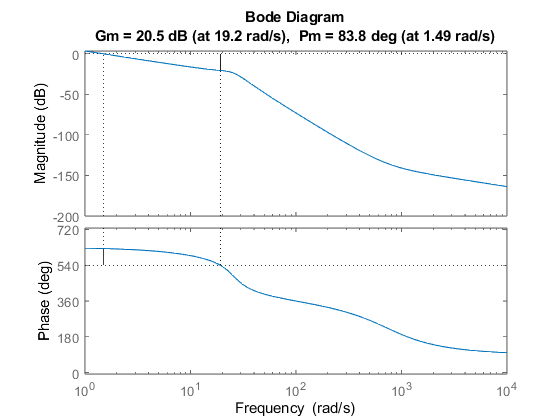
\includegraphics[width=\textwidth]{./images/Chapter 4/FB/Bode_uncontrolled.png}
     \end{subfigure}
     \hfill
     \begin{subfigure}{0.47\textwidth}
         \centering
         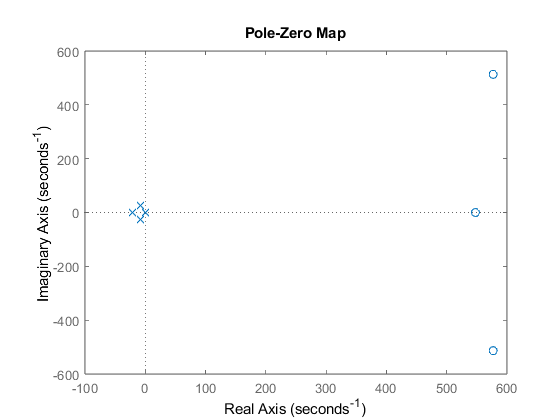
\includegraphics[width=\textwidth]{./images/Chapter 4/FB/pzmap.png}
     \end{subfigure}
\end{figure}


As we did for the base, we cancelled the two complex conjugate poles to reduce the oscillations in the controlled system and added an integrator to grant zero steady state error. This time there are no limitation regarding the speed of the controller due to the absence of the anti-resonance, so theoretically we could speed up the system up to $\approx \omega_{crit}$. As our main goal was to reduce the overshoot of the tip, we opted for a slower, more conservative design.

\begin{equation*}
    C = 51.28 \frac{(s+7.43-24.5i)(s+7.43+24.5i)(s+1)}{s(s+100)^2}
\end{equation*}

We introduced a zero just before the crossing frequency, like we did for the controller of the base, to boost the phase margin, in order to meet our specifications, whereas the two high frequency poles were added for feasibility reasons. The gain was found in such a way to get the maximum possible phase margin and a bandwidth in the order of $\approx 5 \, \frac{rad}{s}$, which is a reasonable trade-off between speed and tip overshoot. 

Here we can see the Bode diagram and the pole-zero map of the open loop controlled system.

\begin{figure}[H]
     \centering
     \begin{subfigure}{0.47\textwidth}
         \centering
         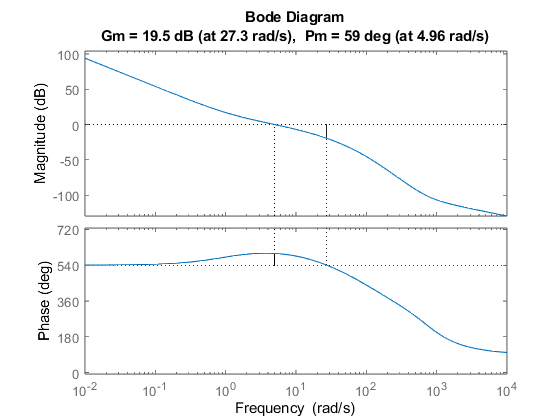
\includegraphics[width=\textwidth]{./images/Chapter 4/FB/Bode_controlled.png}
     \end{subfigure}
     \hfill
     \begin{subfigure}{0.47\textwidth}
         \centering
         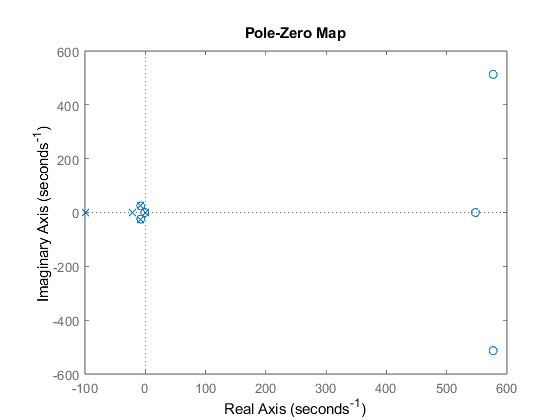
\includegraphics[width=\textwidth]{./images/Chapter 4/FB/pzmap_controlled.png}
     \end{subfigure}
\end{figure}

The overall scheme is then:

\image[1]{./images/Chapter 4/FB/Scheme.png}  

\subsection{Validation}

\subsubsection{Step response}

Below we can see on the left the step response of the controlled system to a 45° reference signal: the tip position quickly increases, the rising time is less than 0.5s, then the integral part of the controller lets the system reach the reference signal in less than 4s.

On the right, instead, we can see the measurements of the $\alpha$ angle, the angle between the arm and the base, which always remains below 4°, which satisfies the assumptions we made regarding the linearization of the system.

\begin{figure}[H]
     \centering
     \begin{subfigure}{0.47\textwidth}
         \centering
         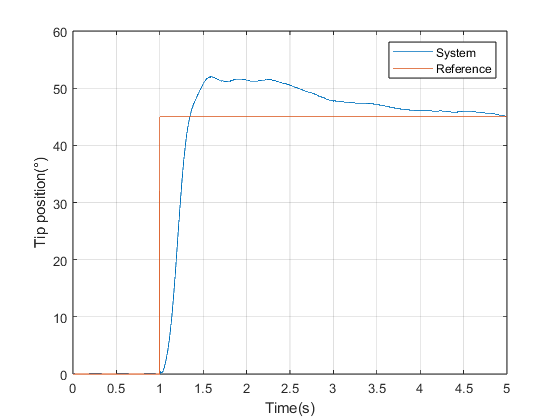
\includegraphics[width=\textwidth]{./images/Chapter 4/FB/Step.png}
     \end{subfigure}
     \hfill
     \begin{subfigure}{0.47\textwidth}
         \centering
         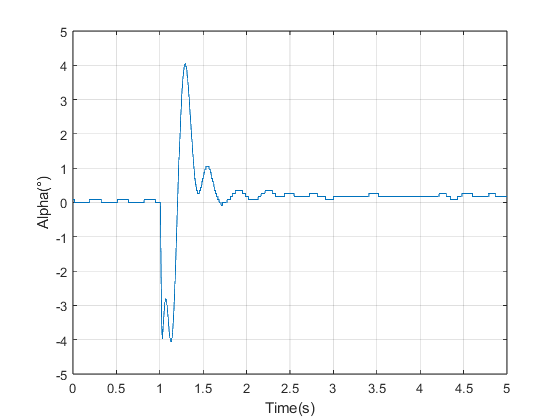
\includegraphics[width=\textwidth]{./images/Chapter 4/FB/Alpha.png}
     \end{subfigure}
\end{figure}

\subsubsection{Frequency validation}

\image{./images/Chapter 4/FB/Tip FB controller Closed Loop.png}   

Finally, once again, we can see how the Bode diagram of the physical system in closed loop matches the expected behaviour.

\section{State Space Based Approach}

To improve the performances of our controlled system we adopted a full state feedback control scheme to able to better change the dynamics of the overall SIMO system.

\subsection{State estimators}

In order to apply such control scheme we must be able to know or estimate the state of our system knowing only its outputs and inputs. For this reason we developed different kinds of state estimators.

To evaluate the performance of each one of them we need to check how correct they are. For this reason we qualitatively compared the states from the estimators with $\theta$ and $\alpha$ available from sensor measurements and their derivatives, $\dot\theta$ and $\dot\alpha$, calculated by the central difference method and smoothed with a Gaussian smoothing filter to remove spikes caused by the differentiation.

\subsubsection{State extractor}

As our output is the array 
$\begin{bmatrix}
    \theta \\
    \alpha
\end{bmatrix}$
and the full state is 
$\begin{bmatrix}
    \theta \\
    \dot\theta \\
    \alpha \\
    \dot\alpha 
\end{bmatrix}$,
we could just apply a derivative to the output to get the full state, as expressed in the simulink scheme below.

\image{./images/Chapter 4/Observers/SE.png}

The benefit of such observer is that the estimation of the state is instantaneous and there is no dynamics for the error between the real and the estimated state.

The main drawback is that the derivative is done numerically, so high frequency noises in the measurements could lead to wrong state estimations.
This can be clearly seen by looking at $\dot\theta$ in the plot below. 
\image{./images/Chapter 4/Observers/Euler.png}


\subsubsection{Luenberger observer}

    In order to provide an estimation for the states we compute an observer that has the goal to imitate the behavior of the system. We obtained the gain of the observer by imposing the poles of the state error dynamics to be ten times faster than the ones of the pole placement, further information in the control section.
                \[
                    s = -230; \qquad s = -250; \qquad s=-270; \qquad s=-290;\]

                To compute the static gain of the observer we used the following matlab command:
\begin{verbatim}
        L_obs = place(sysest.A',sysest.C', obs_poles)';
\end{verbatim}
                
                The Simulink scheme is then:

                \image{./images/Chapter 4/Observers/StateObserver.png}

                The dynamics of the observer is not affected by the saturation limits of the control signal, for this reason we were able to place the dominant pole at such high frequency, which grants a fast enough estimation of the states.
                
                The main drawbacks of this estimator are the need of a perfect knowledge of the system and the low reliability in case of unknown noises, disturbances and uncertainties.
\image{./images/Chapter 4/Observers/Luenberger Observer.png}

            \subsubsection{Kalman filter}

                Lastly we used an optimal observer, namely a Kalman filter, to optimize the estimated state considering noise on the measurements and external disturbances on the output. 

               Measurement noise refers to the inherent uncertainty or errors in the measured output of a system. It captures the discrepancy between the actual output of the system and the output predicted by the model. 
               
               This kind of noise can arise due to various factors such as measurement inaccuracies, sensor noise, or unmodeled dynamics. In our case, our sensors are positional encoders with high resolution and high sampling time. This leads to pretty good measurements with low variance.
\\
\\
Resolution of encoder: $\frac{2\pi}{4096} = 0.0015$\\
Variance of measurement:  $0.0015^2  = 2.25 \times 10^{-6}$\\
\[ 
    R = 
       \begin{bmatrix}
        2.25 \times 10^{-6}
       \end{bmatrix}
       \]

We can assume the same variance on the state as well, by supposing the state to be measured with the same encoders: 

\[ 
    Q = 2.25\times 10^{-6} \times
       \begin{bmatrix}
        1&0&0&0\\
        0&1&0&0\\
        0&0&1&0\\
        0&0&0&1\\
       \end{bmatrix}
       \]

       For the computation of the Kalman filter's static gain we used the command:
       \begin{verbatim}
           L_KF = lqr(sysest.A.', sysest.C.', Q_KF, R_KF).'
       \end{verbatim}



                The Simulink Scheme:

                \image{./images/Chapter 4/Observers/KalmanFilter}

    As we saw, the Kalman filter is an optimal observer, which means that it's able to estimate the states even when the system is subjected to disturbances, but it relies on Gaussian noises with known average and variance and also a good knowledge of the system to estimate.
    Theoretically it is more precise than the Luenberger observer, but also more computationally heavy.
    
\image{./images/Chapter 4/Observers/Kalman Filter Estimator.png}

\subsubsection{Comparison}

To sum everything up, here is the numerical comparison of the three different estimators. The ground truth of states for each time step is $x_{gt}$, each estimator is represented as $x_{estimator}$. N is the number of data samples in the validation dataset. Units of the states are in degrees and degrees per seconds.

    \[
    error =\frac{1}{N}\sum_{k=1}^{N} \left|x_{gt}(k) - x_{estimator}(k)\right|
        \]

\begin{table}[ht]

    \centering
    \caption{Mean absolute error between Ground truth vs Estimators}
    \begin{tabular}{|c|c|} 
    \hline
    State extractor & 5.8855\\ 
    \hline
    Kalman filter & 3.1898\\
    \hline
    Luenberger observer & 1.7703 \\ 
    
 \hline
    \end{tabular}
\end{table}
The state extractor has the largest error due to derivative operation which causes sudden spikes in the estimation. On the other hand, the Kalman filter has smoother behavior but has a shift in the estimation of $\dot\theta$.


\section{Pole Placement}
Pole placement is a control technique used to design a controller that can shape the response of a system by placing its poles at desired locations in the complex plane.
The control law of the pole placement controller is:

\begin{equation*}
    u = -K_{PP}x
\end{equation*}

The controller gain matrix $K_{PP}$ can be calculated with the Ackermann formula by specifying the desired pole locations in the complex plane.
The overall state of the system, or its estimation, is needed for the implementation of this control scheme.
\subsection{Controller design}

The control scheme is the following:

\image{./images/Chapter 4/PP/Scheme.png}

In order to remove the oscillations in the controlled system we decided to place all the poles on the real axis.
We wanted to reduce as much as possible the overshoot of the tip with respect to the base both for design choices and also to grant the validity of our linear model. By doing so we chose to place the dominant pole at $\omega_{dom} = 23 \, \frac{rad}{s}$ and the other poles at higher frequencies. 

\begin{equation*}
    Poles_{PP}= [-23, -25, -27, -29]
\end{equation*}

In this way the controlled system is faster than the uncontrolled one, but is well below the limit introduced by $\omega_{crit}$ (obtained in section \ref{sec: control limits}); in fact we could make the system faster, but doing so the overshoot was no more negligible, for this reason we preferred a more conservative controller.

Using Ackermann's formula we got the following gain:
  
\begin{equation*}
    K_{PP}= [21.1801, 2.6433, -34.8132, 1.3692]
\end{equation*}

When using a pole placement controller, it is sometimes necessary to introduce a scaling term to the reference value in order to reach it effectively. This scaling term ensures that the control control input generated by the controller matches the magnitude and dynamics of the reference signal.


\begin{equation*}
    \begin{cases}
        K_{dc} = D+CA^{-1}B \\
        K_r = \frac{1}{K_{dc}(1)} 
    \end{cases}
\end{equation*}

Using the continuous-time DC gain equation above and inverting it to get the scaling term, we got $K_r$ = 21.1801.

\subsection{Validation}

\subsubsection{Step response}

As we can see, the system is able to perfectly reach the reference with negligible oscillations and without overshooting, also the $\alpha$ angle always remains inside the linearization limits.
\begin{figure}[H]
     \centering
     \begin{subfigure}{0.47\textwidth}
         \centering
         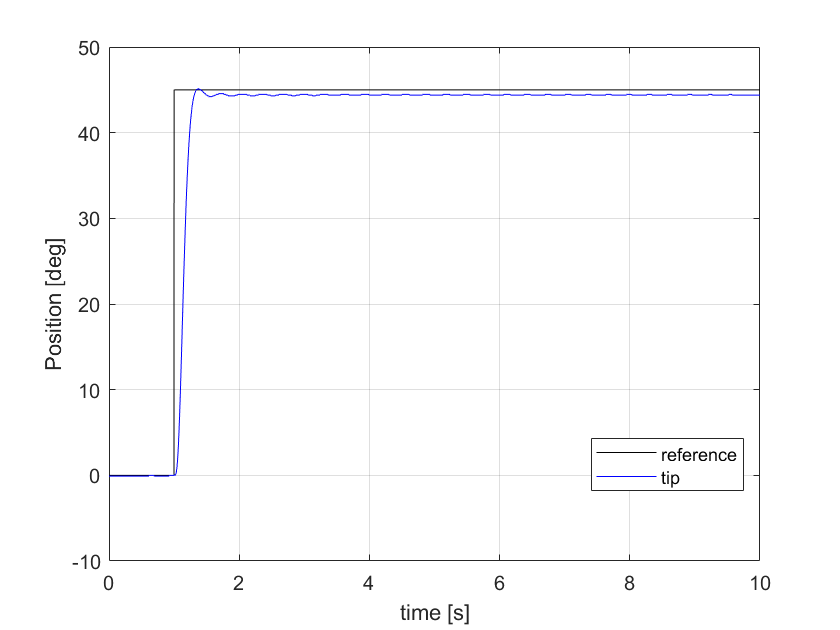
\includegraphics[width=\textwidth]{./images/Chapter 4/PP/ppsteptip.png}    %TODO add images for PP!
     \end{subfigure}
     \hfill
     \begin{subfigure}{0.47\textwidth}
         \centering
         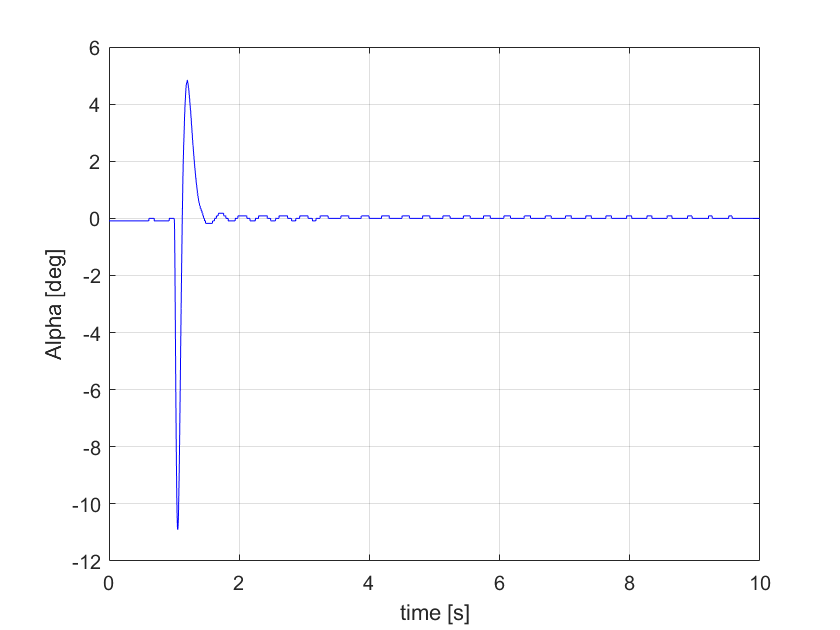
\includegraphics[width=\textwidth]{./images/Chapter 4/PP/ppstepalpha.png}
     \end{subfigure}
\end{figure}
\subsubsection{Frequency validation}
By testing the closed loop system at different sinusoidal input we were able to reconstruct the Bode plot of the system with a pole placement controller.

\image{./images/Chapter 4/PP/Tip PP controller Closed Loop.png}

As can be seen, the model simulates very well the results obtained at low frequency in the real system.


\section{Linear Quadratic Regulator}

The LQ regulator is an optimal full state feedback control scheme which has as control law:

\begin{equation*}
    u = -K_{LQR}x
\end{equation*}

Where $K_{LQR}$ is found by solving this minimization problem:


$$ \min _{u(\cdot)} \int_0^{t_1}\left(x^T Q x+u^T R u\right) d t $$ 
subject to $\dot{x}=A x+B u$ 

Where Q and R are matrices which represent respectively the weight on the state and on the inputs.

\subsection{Controller design}

We implemented a Linear Quadratic Regulator with an integral action in an outer feedback loop, in this way the LQ will provide stability and the integral action will provide a zero steady state error between the tip position and the reference.

The control scheme is the following:

\image[1]{./images/Chapter 4/LQR/LQR_anti_wind_up.png}

To mitigate possible issue related to the saturation limit and the integral action of the enlarged system we also implemented an anti wind-up configuration.

In order to speed up the response of the system we designed the LQ controller by prescribing a convergence rate faster than an exponential:
\[
y =  e^{-\tau t} \]
To do so we added a weight on the A matrix as follows:
\[
    \tilde{A} = A + \tau I\]
In this way we imposed the real part of all the poles of the controller to be smaller than $ -\tau$.

At first we defined the Q and R matrices as identity matrices and tested different values of $\tau$ to see how they would impact the response of the overall system.

\begin{equation*}
Q = 
    \begin{bmatrix}
    1 & 0 & 0 & 0 & 0 \\
    0 & 1 & 0 & 0 & 0 \\
    0 & 0 & 1 & 0 & 0 \\
    0 & 0 & 0 & 1 & 0 \\ 
    0 & 0 & 0 & 0 & 1
\end{bmatrix} 
\qquad 
R = 1
\end{equation*} 

These results are obtained with a step response for the tip of 45°:
\begin{itemize}
    \item $\alpha$ overshoot [\%] ($\alpha$ OS);
    \item Tip overshoot [\%](Tip OS);
    \item Settling Time [s](ST);
    \item Rising Time [s](RT);
    \item Max Control Variable [V](Max V);
    \item Integral of the Control Variable [Vs](I V);
    
\end{itemize}

\begin{table}[h!]
    \centering
    \hspace*{-3em}
    \begin{tabular}{||c c c c c c c||} 
    \hline
    $\tau$ & $\alpha$ OS & Tip OS & ST & RT & Max V & I V\\ 
    \hline\hline
    15 &  11.405 & 0.000 & 0.732 & 0.158 & 6.315 & 0.528 \\ 
    \hline
    17 &  12.725 & 0.000 & 0.611 & 0.152 & 8.050 & 0.528 \\ 
    \hline
    20 & 15.268 & 0.000 & 0.455 & 0.144 & 11.905 & 0.537 \\ 
    \hline
    25 & 25.194 & 0.000 & 0.301 & 0.108 & 59.267 & 2.432 \\ 
    \hline
    \end{tabular}
\end{table}
\image{./images/Chapter 4/LQR/LQR_Tau_comparison.png}   

In the plot above we can clearly see how increasing $\tau$ we can have a faster response, but also the control signal required increases as well, going over the saturation limits.

By choosing $\tau = 20$ we can mitigate the trade-off between fast response and saturation limits.

For this value of $\tau$ we noticed that changing the weights on the main diagonal of the Q matrix doesn't have an impact on the performances of the controlled system, so we kept them as identity matrices.

Their contribution start to be relevant for lower values of $\tau$, but as the response of the system was too slow in that configuration we decided to keep the value of $\tau = 20$.

\subsection{Validation}
\subsubsection{Step response}
Below we can see on the left the step response: the rising time is less than 0.13s and the settling time is slightly more than 0.5 seconds. On the right, instead, we can see the measurements of the $\alpha$ angle which has a couple of big peak, the highest of 17°, which still satisfies the assumptions we made regarding the linearization of the system.

\begin{figure}[H]
     \centering
     \begin{subfigure}{0.47\textwidth}
         \centering
         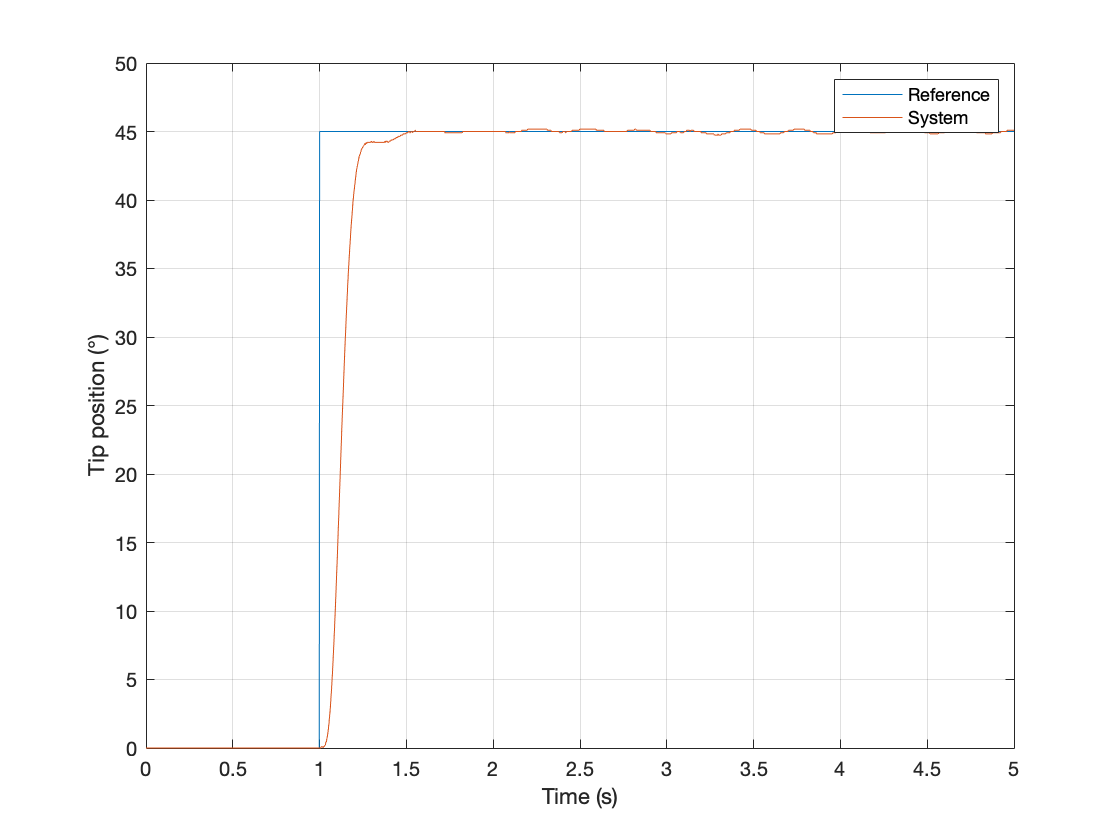
\includegraphics[width=\textwidth]{./images/Chapter 4/LQR/Step.png}
     \end{subfigure}
     \hfill
     \begin{subfigure}{0.47\textwidth}
         \centering
         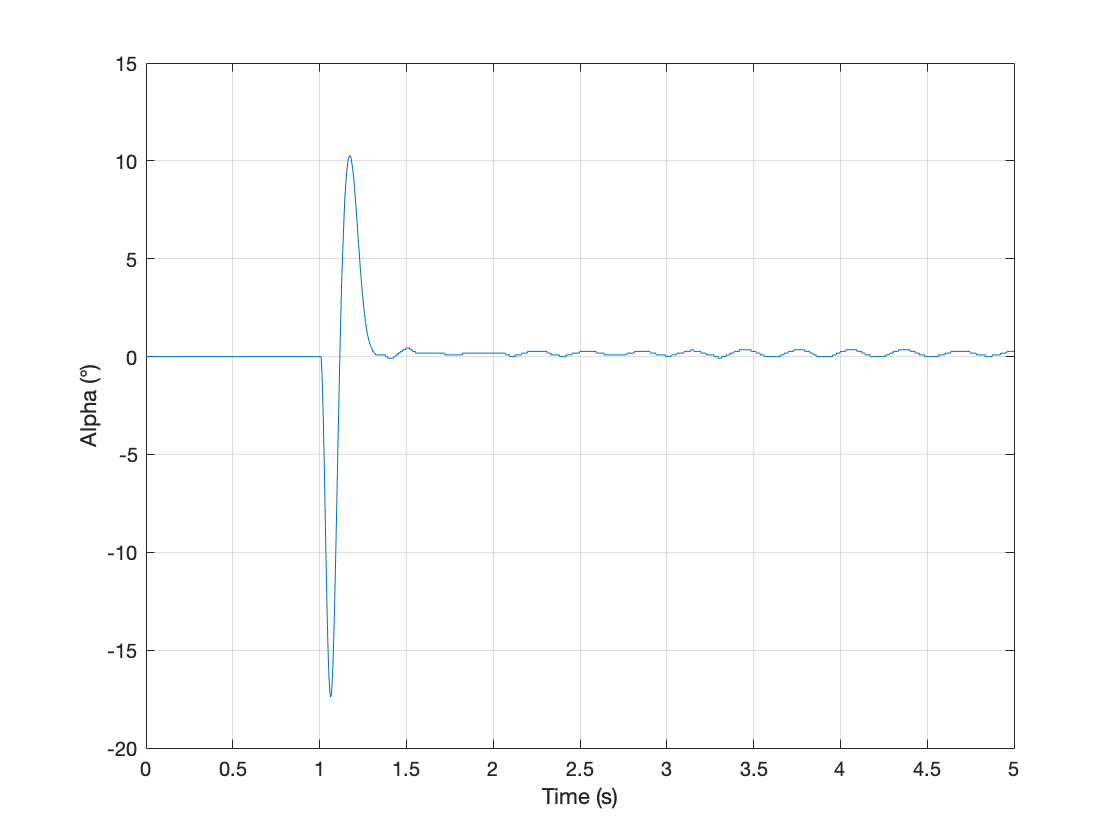
\includegraphics[width=\textwidth]{./images/Chapter 4/LQR/Alpha.png}
     \end{subfigure}
\end{figure}


\section{Comparison}

To decide which controller to use, we compared their performances with a step response.

\begin{figure}[H]
     \centering
     \begin{subfigure}{0.47\textwidth}
         \centering
         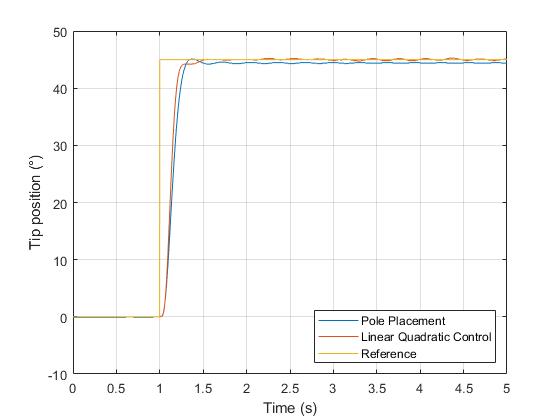
\includegraphics[width=\textwidth]{./images/Chapter 4/Comparison/Step.png}
     \end{subfigure}
     \hfill
     \begin{subfigure}{0.47\textwidth}
         \centering
         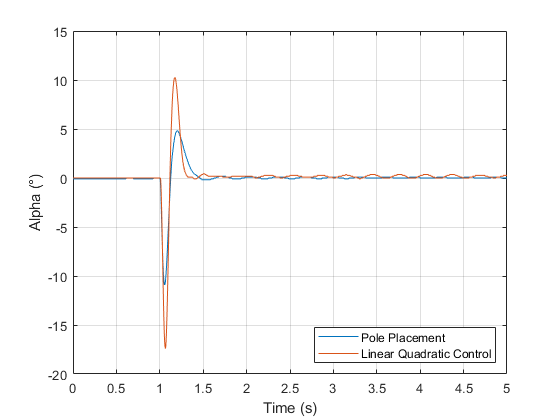
\includegraphics[width=\textwidth]{./images/Chapter 4/Comparison/Alpha.png}
     \end{subfigure}
\end{figure}

The main features are:


\begin{table}[h!]
    \centering
    \hspace*{-3em}
    \begin{tabular}{||c c c c c c c||} 
    \hline
    Method & $\alpha$ OS & Tip OS & ST & RT & Max V & I V\\ 
    \hline\hline
    PP &  11.405 & 0.000 & 0.791 & 0.172 & 16.298 & 0.977 \\ 
    \hline
    LQR & 15.268 & 0.000 & 0.455 & 0.144 & 11.905 & 0.537 \\ 
    \hline
    \end{tabular}
\end{table}

Both the control schemes have a settling time lower than one second and a similar rising time, however we prefer the performances of the pole placement controller because the $\alpha$ overshoot is less.